\subsection{Use Case}

I \textbf{Use Case Diagram} servono per identificare le funzionalità svolte dal sistema software. Queste devono essere assegnate a oggetti/classi (\textbf{assegnazione di responsabilità}). Si parte dalle macro-funzionalità, raffinandole fino ad arrivare a operazioni che non ammettono ulteriore decomposizione. Eventuali ambiguità possono essere chiarite tramite \textit{Activity Diagram}. L'analisi dei casi d'uso può:
\begin{itemize}
    \item aiutare a identificare gli oggetti;
    \item definire i casi di test dei moduli;
    \item descrivere le dinamiche di interazione con il sistema.
\end{itemize}

\begin{figure}[H]
    \centering
    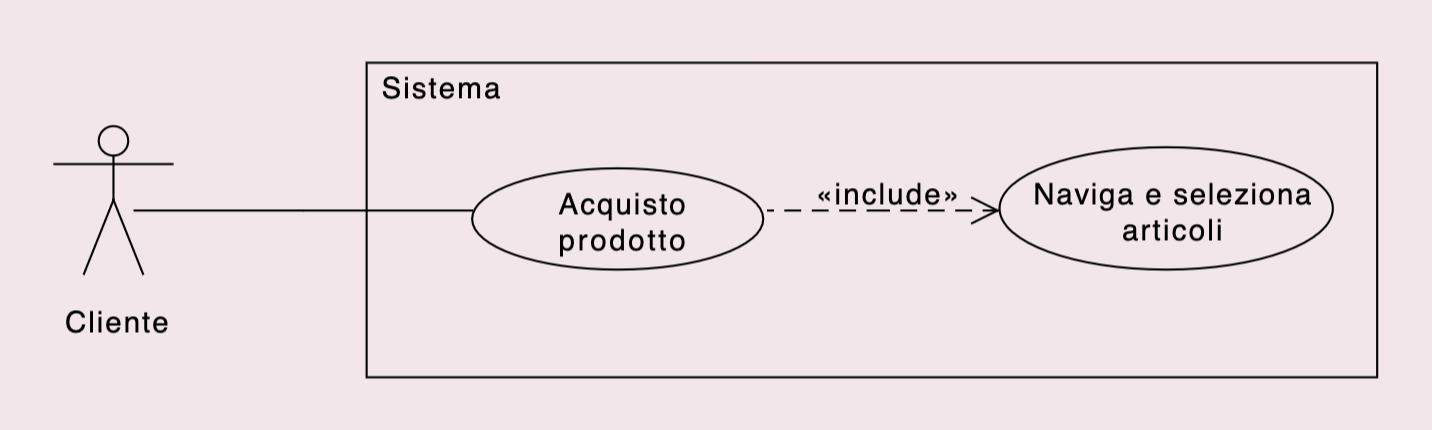
\includegraphics[width=0.75\linewidth]{assets/UML/use-case/use-case1.png}
    \caption{Esempio di Use Case Diagram}
    \label{fig:use-case1}
\end{figure}

\paragraph{Attore} Rappresenta un ruolo interpretato da entità esterne (utenti o sistemi). L'\textbf{attore principale} è colui che persegue lo scopo del caso d'uso (gli altri sono secondari). Sussiste una relazione molti-a-molti tra attori e casi d'uso.

\textbf{\textit{Rappresentazione}}: omino stilizzato.

\paragraph{Scenario} Sequenza di passi che caratterizza l'interazione complessa tra un attore e il sistema software stesso. In particolare si distinguono:
\begin{itemize}
    \item \textbf{Main scenario}: scenario principale di successo (obiettivo raggiunto);
    \item \textbf{Scenari secondari} (o estensioni del main): divergono dal main scenario o sono contenuti in esso (possono o meno raggiungere lo scopo prefissato).
\end{itemize}
\textbf{\textit{Rappresentazione}}: rettangolo contenente i casi d'uso dello scopo.

\paragraph{Caso d'uso} Insieme di scenari che hanno lo stesso scopo finale (per l'utente). Uno scenario è una possibile "esecuzione" (istanza) del caso d'uso. Può comprendere:
\begin{itemize}
    \item \textbf{Pre-condizioni}: descrivono ciò che il sistema deve assicurare prima che il caso d'uso possa avere inizio;
    \item \textbf{Garanzie}: descrivono ciò che il sistema deve assicurare alla fine dello svolgimento del caso d'uso;
    \item \textbf{Trigger}: specificano l'evento che dà origine al caso d'uso.
\end{itemize}
\textit{Alastair Cockburn} suddivide i casi d'uso in tre livelli:
\begin{itemize}
    \item \textbf{Kite-level}: mostrano come più sea-level portano all'interazione tra diversi attori (livello superficiale);
    \item \textbf{Sea-level}: interazioni attore principale/sistema (livello mediano);
    \item \textbf{Fish-level}: esistono perché inclusi in un sea-level (livello profondo).
\end{itemize}
Un passo di caso d'uso corrisponde a un'interazione tra attore e sistema; è descritto da una frase semplice e non esprime dettagli tecnici.

\textbf{\textit{Rappresentazione}}: ellisse contenente il nome del caso d'uso.

\begin{figure}[H]
  \centering
  \subfloat[Generalizzazione tra casi d'uso: il caso d'uso figlio "specializza" (estende) alcuni aspetti del padre]{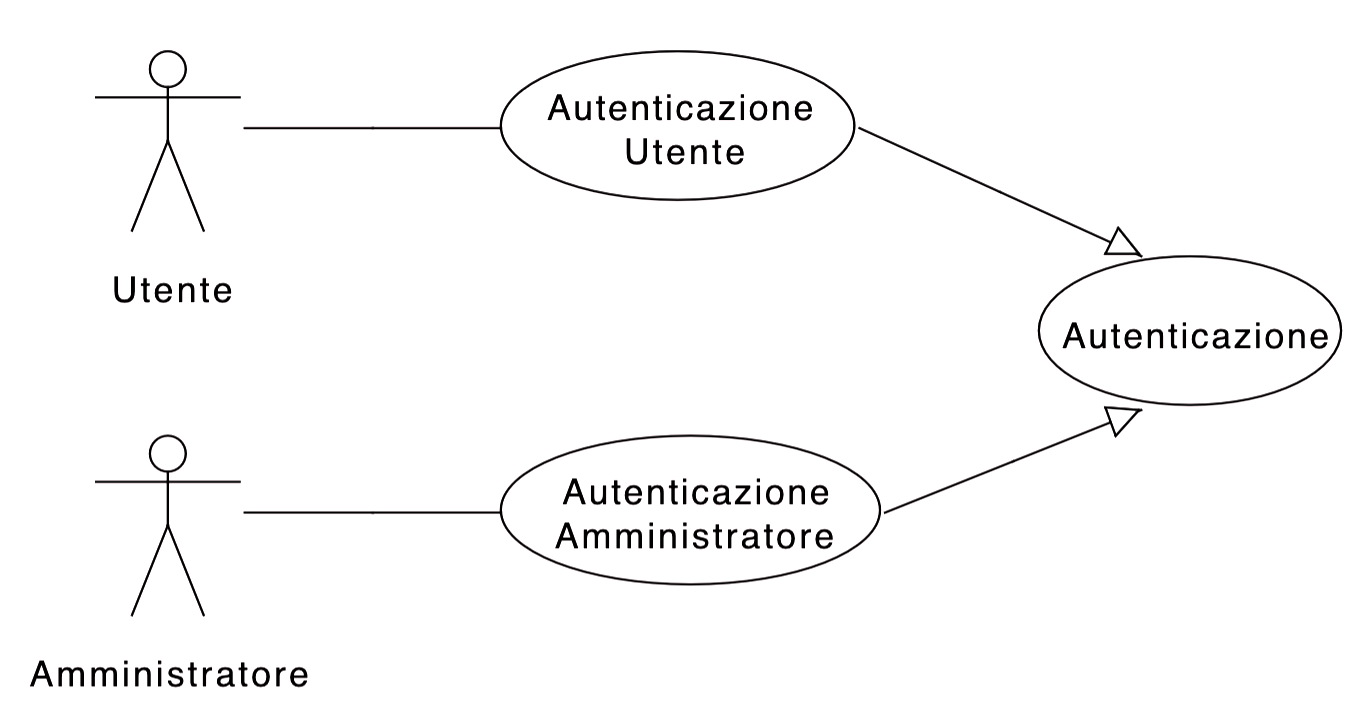
\includegraphics[width=0.575\linewidth]{assets/UML/use-case/use-case2.png}}
  \hfill
  \subfloat[Generalizzazione tra attori: ruolo figlio più specifico, \textit{compatibile} con il ruolo padre]{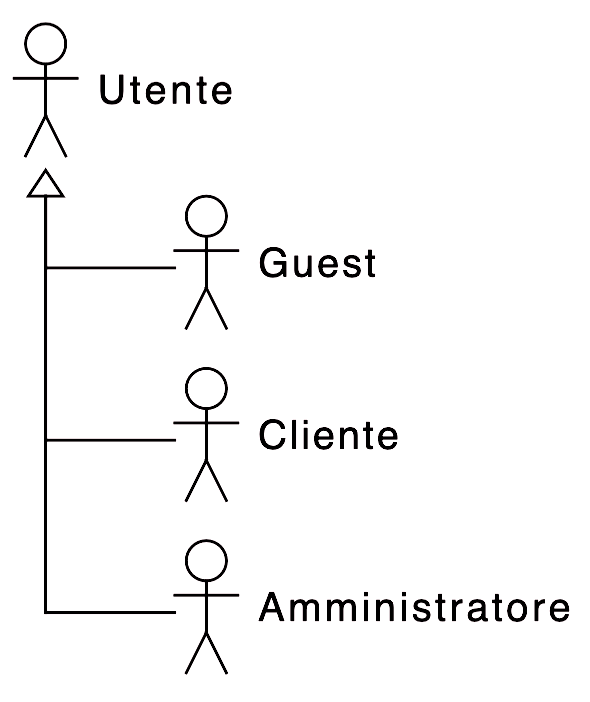
\includegraphics[width=0.25\linewidth]{assets/UML/use-case/use-case3.png}}
\end{figure}

\subparagraph{Estensione} Condizione che determina il verificarsi di interazioni diverse dallo scenario principale. Si indicano: il passo in cui si verifica la condizione, i passi (numerati) che descrivono le interazioni dell'estensione e (se necessario) il punto di rientro nello scenario principale.\\
\textbf{\textit{Rappresentazione}}: linea tratteggiata che termina con una freccia etichettata con la parola chiave $\langle\langle$extend$\rangle\rangle$.

\begin{figure}[H]
  \centering
  \subfloat[Relazione di estensione]{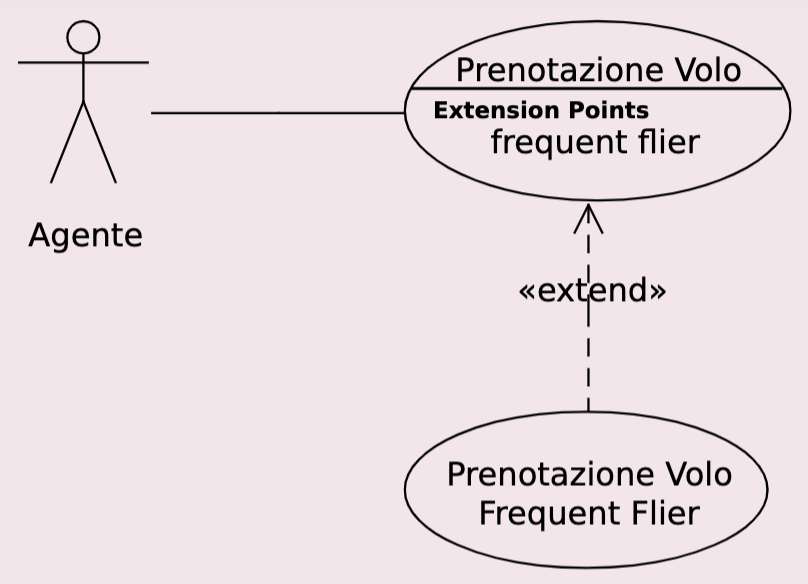
\includegraphics[width=0.41\linewidth]{assets/UML/use-case/use-case5.png}}
  \hfill
  \subfloat[Esempio di caso d'uso in forma testuale]{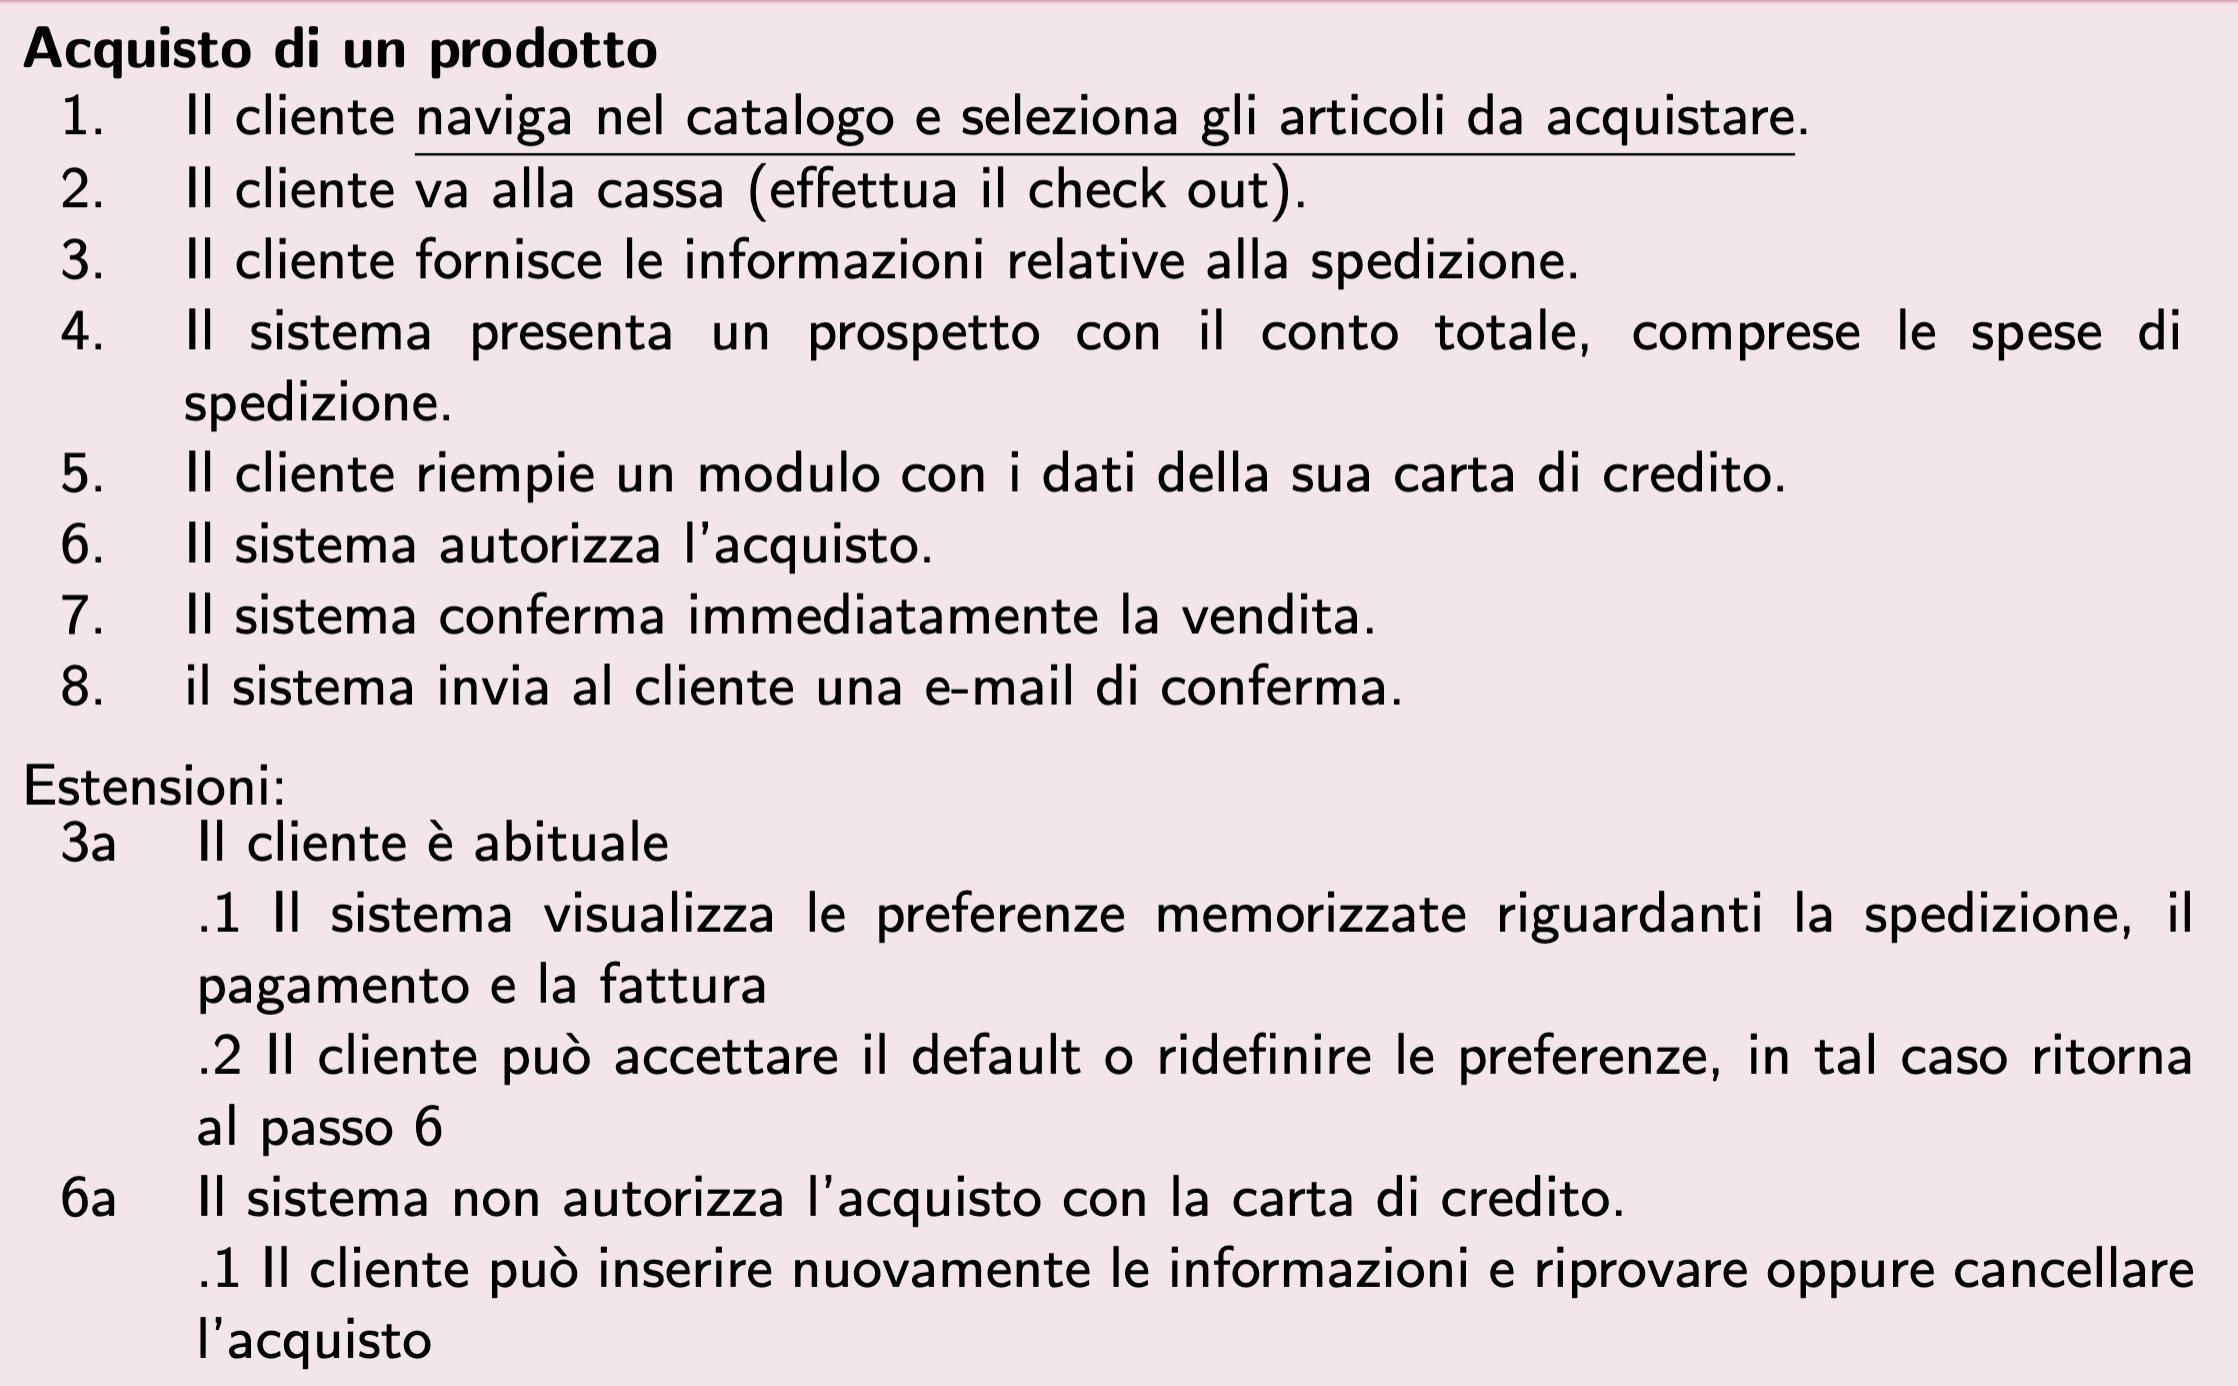
\includegraphics[width=0.48\linewidth]{assets/UML/use-case/use-case4.png}}
\end{figure}

\subparagraph{Inclusione} Scissione di un passo di un caso d'uso complicato, espresso come un altro caso d'uso completo (il primo \textit{include} il secondo). In forma testuale è sufficiente sottolineare il nome del caso d'uso incluso.

\textbf{\textit{Rappresentazione}}: linea tratteggiata che termina con una freccia (dipendenza) etichettata con la parola chiave $\langle\langle$include$\rangle\rangle$.

\newpage